The NR-IQA method provided a sharpness measure for each image of the datasets and such numerical representations were analyzed with the $z$-score; at this point, the estimate of eligible images was prompted to the user and the real eligible ones were chosen. The obtained subset is registered by means of the SIFT-based z-stack alignment tool of the TrakEM2 package. The subsequent stage is to perform the fusion of images in the before-mentioned subset. We propose a multifocus bright-field microscopy image fusion algorithm with the Laplacian of Gaussian edge detection filter and the energy of edges. Fig.~\ref{fig:fusion_pipeline} shows a diagram of the proposed method.

\begin{figure}[ht]
    \centering
    \caption{Diagram of the proposed multifocus bright-field microscopy image fusion algorithm.}
    \label{fig:fusion_pipeline}
    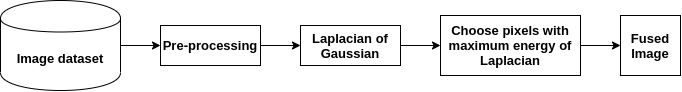
\includegraphics[scale=0.65]{images/fusion_pipeline.png}
    \centering
    \fautor
\end{figure}

The grayscale version of the selected images is again used for fusion; since the images were converted with the luminance method, the edges are preserved and therefore the edge detection may be successful. Other methods from the \emph{Luminance} family, e.g. \emph{Luminance}, \emph{Luminance\'}, \emph{Luma} and \emph{Decolorize}, are also suitable \cite{kanan2012color}.

The images then undergo the Laplacian of Gaussian filter - a spatial filtering algorithm that extracts edges of a smoothed image. The Laplacian is a second-order derivative isotropic linear operator, based on the Laplacian of a function, which defines an edge as the zero-crossing of the second derivative of a function. First and foremost, the Laplacian of a function is denoted by

\begin{equation}
\label{eqn:laplacian_of_function}
\nabla^{2}g(x,y) = \frac{\partial^{2} g(x,y)}{\partial x^{2}}
                    +
                  \frac{\partial^{2} g(x,y)}{\partial y^{2}},
\end{equation}

\noindent where $g(x,y)$ is the input image. For the discrete case (which applies to the digital images), the Laplacian operator is achieved by means of a convolution. The approximation of the second derivatives in each dimension yields the following convolution kernel

\begin{equation*}
\label{eqn:discrete_laplacian}
\begin{bmatrix}
0 & 1 & 0 \\
1 & -4 & 1 \\
0 & 1 & 0
\end{bmatrix}.
\end{equation*}

Similarly, instead of extracting edges with the Laplacian filter only, the Laplacian of Gaussian filter performs a Gaussian filtering process to remove noise and smooth the images before retrieving the edges \cite{marr1980theory}. This approach applies to cases where the quality and reliability of edges obtained by the Laplacian operator are sensitive to noise, and also plays the role of distinguishing the blurry regions from the sharp ones in our approach; pixels belonging to sharp regions will suffer a stronger smoothing effect in comparison to blurry pixels. For our application, an image is convolved with a two-dimensional Gaussian filter, denoted by

\begin{equation}
\label{eqn:gaussian_filter}
S(x,y) = g(x,y) \ast \frac{1}{\sqrt{2 \pi \sigma}} e^{- \frac{x^{2} + y^{2}}{\sigma^{2}}},
\end{equation}

\noindent where $S(x,y)$ is the smoothed version of the image, $g(x,y)$ is the input image and $\sigma$ is the standard deviation of the Gaussian function. Then, the Laplacian is applied to the smoothed image $S$. Both operators are linear and shift-invariant and therefore can be applied in any order, but the Gaussian filter is commonly applied first if the application required separated filters. In our case, the Laplacian of Gaussian operator can be defined as

\begin{equation}
\label{eqn:laplacian_of_gaussian}
LoG(x,y) = - \frac{1}{\pi \sigma^{4}}
            \left[
                1 - \frac{(x^{2} + y^{2})}{2 \sigma^{2}}
            \right]
            e^{- \frac{x^{2} + y^{2}}{2 \sigma^{2}}}.
\end{equation}

\noindent The $\sigma$ parameter is responsible for the smoothing magnitude. The convolution kernel is then a combination of both Laplacian and Gaussian filters; higher $\sigma$ values increase the effective kernel size consequently the smoothing effect. The next step is to retrieve the energy for each region, also based on the fact that blurry regions of an image present less high-frequency components than sharp regions. This stems from the fact that sharp regions are prone to have more edges than smoothed ones, hence a higher energy level. The higher the number the edges in an area of the image, the better the focus on it. Therefore, pixels that correspond to edges are chosen to form the fused image. Their spatial location is used to construct an RGB image by retrieving the content of the three channels from those pixels and assigning them to the final image.